%        File: HW4.tex
%     Created: Wed Feb 16 01:00 PM 2011 C
% Last Change: Wed Feb 16 01:00 PM 2011 C
%
\documentclass[10pt,letterpaper]{article}
\usepackage{amsmath,amsfonts,amssymb}
\usepackage[]{graphicx}
\usepackage{cancel}
\usepackage{listings}
\usepackage[]{color}
\usepackage{textcomp}
\definecolor{listinggray}{gray}{0.9}
\definecolor{lbcolor}{rgb}{0.9,0.9,0.9}
\lstset{
	backgroundcolor=\color{lbcolor},
	tabsize=4,
	rulecolor=,
% 	language=Python,
        basicstyle=\scriptsize,
        upquote=true,
        aboveskip={1.5\baselineskip},
        columns=fixed,
        showstringspaces=false,
        extendedchars=true,
        breaklines=true,
        prebreak = \raisebox{0ex}[0ex][0ex]{\ensuremath{\hookleftarrow}},
        frame=single,
        showtabs=false,
        showspaces=false,
        showstringspaces=false,
        identifierstyle=\ttfamily,
        keywordstyle=\color[rgb]{0,0,1},
        commentstyle=\color[rgb]{0.133,0.545,0.133},
        stringstyle=\color[rgb]{0.627,0.126,0.941},
}
\renewcommand*\arraystretch{1.2}
\addtolength{\parskip}{\baselineskip}

\def\mbf{\mathbf}
\def\mbb{\mathbb}

\providecommand{\abs}[1]{\left\lvert#1\right\rvert}
\providecommand{\norm}[1]{\left\lVert#1\right\rVert}
\def\d{\mathrm{d}}
\def\e{\mathrm{e}}

\title{Numerical Treatment of Differential Equations: Homework 4}
\author{Truman Ellis}
\begin{document}
\maketitle

\section*{Problem 1}
Compute the domain of linear stability for the RK2 scheme:
\[
y_{n+1}=y_n+\frac{h}{2}\left[ f(t_n,y_n)+f(t_{n+1},y_n+hf(t_n,y_n))\right]\,.
\]

\subsection*{Solution}
First we write out the tableu for this method:
\[
\begin{array}{c|c}
    \mbf{c} & A\\
    \hline
    & \mbf{b}^T
\end{array}=
\begin{array}{c|cc}
    0 & 0 & 0\\
    1 & 1 & 0\\
    \hline
    &\frac{1}{2}&\frac{1}{2}
\end{array}\,.
\]
Now 
\begin{align*}
p(z)&=1+z\mbf{b}^T(\mbf{I}-z\mbf{A})^{-1}\mbf{1}\\
&=1+z\mbf{b}^T\left(
\begin{array}{cc}
    1 & 0\\
    -z & 1
\end{array}\right)^{-1}\mbf{1}\\
&=1+z\left(\frac{1}{2}\,,\,\frac{1}{2}\right)\left(
\begin{array}{cc}
    1 & 0\\
    z & 1
\end{array}\right)\left(
\begin{array}{c}
    1\\
    1
\end{array}\right)\\
&=1+z+\frac{1}{2}z^2\,.
\end{align*}
Now we wish to find 
\[
\abs{p(z)}=\abs{1+z+\frac{1}{2}z^2}<1\,.
\]
Using Mathematica, we were able to plot this region as shown in Figure 1.
\begin{figure}[h]
    \begin{center}
        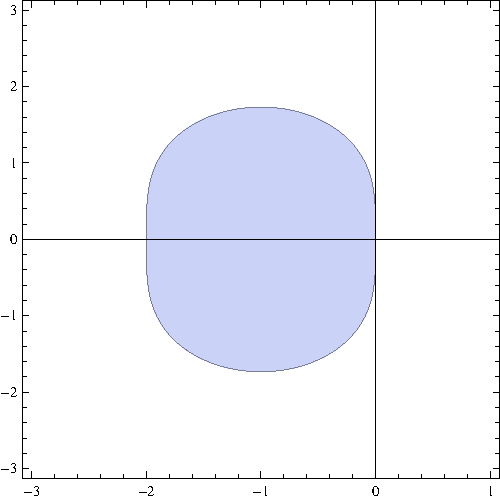
\includegraphics[width=5in,keepaspectratio]{P1.pdf}
    \end{center}
    \caption{Domain of linear stability is the interior of the plotted region}
    \label{fig:P1}
\end{figure}
% Indeed, evaluating
% \[
% \abs{p(-1)}=\abs{\frac{1}{2}}<1\,.
% \]

\section*{Problem 2}
\subsection*{Part a}
\paragraph{(i)}For $0\leq t\leq 1$ and $h=0.1$, the Euler method produced a log error of $8.8499e+00$ 
while the backward Euler method only produced a log error of $-4.0362e+00$.
\paragraph{(ii)}For $0\leq t\leq 10$ and $h=0.01$, the Euler method produced a log error of $-6.2941e+00$ 
while the backward Euler method only produced a log error of $-6.3025e+00$.

The stiffness ratio for this system is 100. By a simple linear stability analysis of the Euler method, we discover
that a time step $0<h< 0.2$ is necessary for stability. Indeed we see this prediction manifested in the results.
With a timestep of 0.1, the Euler method diverges radically from the exact solution. When we reduce the time step 
to the acceptable range, we see dramatic improvement in the error.

The backward Euler method on the other hand carries no timestep restrictions for stability and we readily see this
in our results. We are able to get somewhat reasonable results for even the larger timestep.

\subsection*{Part b}
\paragraph{(i)}For $h=0.05$, the Euler method produced a log error of $5.1083e-01$ while the 
backward Euler only produced a log error of $-3.6031e-01$.
\paragraph{(ii)}For $h=0.2$, the Euler method produced a log error of $1.6608e+01$ while the 
backward Euler only produced a log error of $5.1083e-01$.

We will be able to study the stability properties of this problem more easily if we linearize it:
\begin{align*}
    \mbf{y}'&=\binom{-y_1^2}{-y_1y_2}=\mbf{f}(\mbf{y})\\
    &\approx\mbf{f}(\mbf{y_0})+\nabla\mbf{f}(\mbf{y_0})(\mbf{y}-\mbf{y_0})\\
    &=\binom{-100}{-100}+\left(
    \begin{array}{cc}
    -20 & 0\\
    -10 & -10
\end{array}\right)\binom{y_1-10}{y_2-10}\,.
\end{align*}
Now we can see that the linearized system has eigenvalues 10 and 20. By a linear stability analysis, the Euler
method needs a timestep $0<h<0.1$. The numerical experiment bears this out. The solution quickly becomes unstable
for $h=0.2$, but we get a reasonable error level when we reduce the timestep to $h=0.05$. Similarly as before,
the backward Euler method has no stability bounds on the timestep and we are able to get reasonable solutions
with both timestep sizes.
\end{document}
